\documentclass[a4paper]{article}
\usepackage{float} 
\usepackage{graphicx} 
\usepackage{hyperref}
\usepackage[spanish]{babel} 
\title{Ejercicio 2}
\begin{document}
   \maketitle 
   Tenemos el problema de que, cuando $\omega > \omega_0$ la ecuación $\left( 1 \right) $ indica que el índice de refracción es menor que 1. Como $n=\frac{c}{v}$ esto quiere decir que $v>c$, en contradicción con la idea que tenemos de que la velocidad de la luz no puede ser superada. A continuación veremos porqué este resultado no entra en conflicto con teorías como la teoría de la relatividad. Para ello hay que definir qué velocidad es realmente la que estamos usando para definir el índice de refracción. Definimos por tanto los siguientes términos:

\begin{itemize}
    \item Velocidad de fase: Velocidad que viaja un punto concreto de la onda.  
    \item Velocidad de grupo: La velocidad de grupo es la velocidad de la envolvente de la onda, es decir, la velocidad a la que se mueve el paquete de un grupo de ondas. Para ver mejor estas definiciones veamos una simulación:
        \begin{figure}[H]
            \centering
            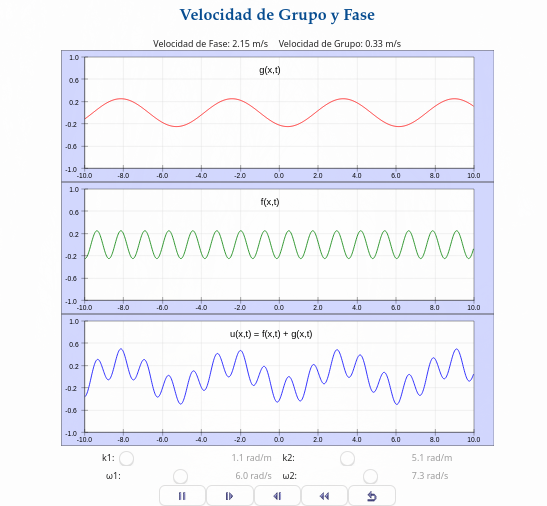
\includegraphics[width=0.8\textwidth]{simulacion.png}
            \caption{Simulación de la uma de dos ondas con diferente $\omega$ (velocidad angular) y $k$ (Número de onda)}
            \label{fig:simulacion-png}
        \end{figure}

\end{itemize}
Tanto la velocidad de fase como la velocidad de grupo pueden superar la velocidad de la luz $c$, haciendo por tanto que el índice de refracción sea $n<1$, veamos porqué ocurre esto y porqué no entra en contradicción con la teoría especial de la relatividad que indica que nada puede viajar más veloz que la velocidad de la luz:\\
\\
Pues bien, realmente lo que nos afirma la teoría especial de la relatividad es que nada con masa en reposo debe viajar más rápido que la velocidad de la luz. Esto también aplica a señales de información, es decir, estas tampoco pueden viajar más allá de la velocidad de la luz, por ello nos preguntamos, ¿Es la velocidad de fase o la velocidad de grupo la velocidad a la que se transmite la información de la onda?, la respuesta es que no. La velocidad de fase no tiene ninguna interpretación física de lo que se transporta en la onda, , por ello, se puede exceder la velocidad de fase por encima de la luz, como veremos más adelante con un experimento teórico investigado por Lijun Wang. \\
\\
Si buscamos en la zona superficial de internet encontraremos que la velocidad de grupo es la velocidad encargada de transmitir la información de la onda, sin embargo, esto no siempre es así. Se suele asociar al pulso máximo con señal (información), sin embargo, la envolvente de la onda puede decaer de forma rápida mediante una atenuación de la intensidad, de forma que la velocidad de grupo sea mayor que la velocidad de la luz. Según Wikipedia, "\textit{La información recibida al llegar un pulso se puede obtener  antes de que llegue el pulso máximo}", pero esto no quiere decir que la velocidad de la información que se transporta sea mayor que la velocidad de la luz.\\
\\
Esto es prueba de que la velocidad de grupo y de fase de la onda puede ser mayor que $c$ bajo ciertas restricciones, siendo por tanto el índice de refracción menor que 1 según la fórmula $n\left( w \right) $. \\
\\
A continuación vamos a ver un experimento llevado a cabo por el físico Lijun Wang llamado \textbf{Detail statement on faster than c light pulse propagation}. En un artículo previo, el investigador afirma que se puede llegar a encontrar una velocidad de fase de 300 veces mayor que la velocidad de la luz, esto es, la velocidad de un pulso al atravesar un átomo (en este caso de Cesio) es mayor que la velocidad de la luz. Este experimento no se puede realizar debido a que se necesita una temperatura de aproximadamente $T\approx 0 K$, algo que no se puede realizar fácilmente en la Tierra.\\
\\
En la siguiente foto vemos que ocurriría con un prisma cuando un rayo de luz le atraviesa y se refracta:
\begin{figure}[H]
    \centering
    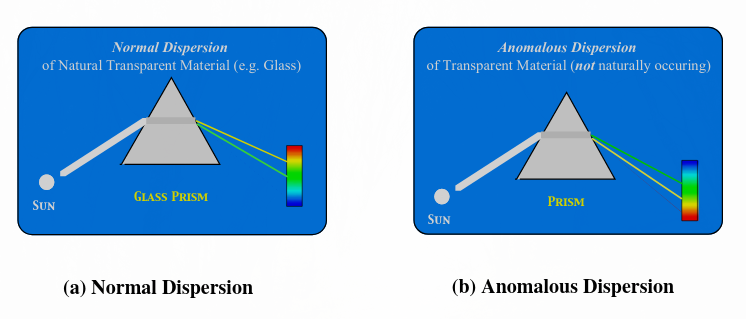
\includegraphics[width=0.8\textwidth]{prisma.png}
    \caption{Dispersión normal a la izquierda, con un $\omega < \omega_0$ y a la derecha dispersión 'anómala' $\omega > \omega_0$}
    \label{fig:prisma-png}
\end{figure}
Vamos a intentar entender el fenómeno que ocurre en el segundo primsa (dispersión anómala) con nuestras ecuaciones:\\
\\
En un rango determinado de frecuencias dado por la frecuencia de resonancias, se tiene que $\frac{dn}{d\omega} <0$, es decir, el índice de refracción disminuye al aumentar la frecuencia. Como la frecuencia del rojo es menor que la del azul, el índice de refracción del rojo es mayor que el del azul, por tanto, la componente roja tiene más ángulo de desviación que la componente azul, tal como vemos en la figura (2.b). \\
\\

Lo aprendido en clase es que hay varios rangos de frecuencias para el cual $\frac{d n}{d \omega} <0$ (El número de rangos de frecuencias viene dado por la cantidad de frecuencias de resonancia que tenga el material, $\omega_0$). Si recordamos, en la clase de teoría vimos que la polarización $\vec{P}$ se define como:
\[
    \vec{P}= \vec{E}\cdot x\left( t \right)     
.\] 
Donde $x\left( t \right) $ era la solución de la ecuación del oscilador armónico $x\left( t \right) = \frac{\frac{q_e}{m_e}}{\left( \omega_0^2-\omega^2 \right) } E\left( t \right) $. Por tanto, si $\omega> \omega_0$ esto quiere decir que el vector de polarización es antiparalelo al campo eléctrico, o lo que es lo mismo, el movimiento oscilatorio del electrón con respecto a la onda incidente del campo eléctrico está desfasado $180^o$ y esto a su vez da lugar a que el índice de refracción sea menor que 1 para ciertos rangos de frecuencias. \\
\\
En conclusión, hemos aprendido con esta tarea que al calcular el índice de refracción no usamos la velocidad de transferencia de información de la onda, la cual no debe pasar la velocidad de la luz; sin embargo la velocidad de grupo y la velocidad de fase si que pueden hacerlo, como ejemplo de esto vemos el experimento llevado a cabo por Lijun Wang. Por tanto, podemos obtener un índice de refracción menor que 1 para distintos rangos de frecuencias según lo visto en clase y no contradice bajo ninguna circunstancia la teoría especial de la relatividad.
\section{Referencias}
\begin{itemize}
    \item[Simulación]: \url{www.kyleforinash.altervista.org/Ondas/GroupVelocityJS.html}
    \item[Medios superlumínicos:] \url{https://es.wikipedia.org/wiki/Superlum\%C3\%ADnico}
    \item[Artículo Lijun Wang:] \url{www.nec.co.jp/press/en/0007/images/1901.pdf}
    \item[Definición $v_f, v_g$]: \url{www.sc.ehu.es/sbweb/fisica_/ondas/interfer/dispersivo/dispersivo.html }
    \item[Ayudas varias:] 1: Hetch. 3.5.; Apuntes de Clase. Tema 7.2
\end{itemize}
\end{document}
